\documentclass[conference]{IEEEtran}
\usepackage{cite,amsmath,graphicx,booktabs,url,array}
\usepackage[T1]{fontenc}
\begin{document}
\title{Detection of Concept Drift in Industrial Data Streams: A Hybrid Drift Trigger Evaluated on Synthetic, IIoT and Live Kafka Streams}
\author{\IEEEauthorblockN{G Jeevan Jadhav (2023BCS0098), K Akhil (2023BCD0018),\\ P Joshua Naik (2023BCS0089), N Mohammed Suhail Ahmed Khan (2023BCS0222)}
\IEEEauthorblockA{IOE413 Streaming Data Analytics, Topic 12}}
\maketitle

\begin{abstract}
Machine-learning models deployed on industrial streams silently lose accuracy when the data-generating process changes (concept drift). We compare the error-rate detectors DDM, EDDM, HDDM-A and HDDM-W, reproducing the benchmark protocol of Sakurai et al., together with ADWIN, and propose a hybrid trigger that fuses HDDM-A and ADWIN with an OR rule and a refractory period. On 480 synthetic streams in three settings the hybrid has the highest mean detection F1 (0.733, 0.786 and 0.591 against 0.672, 0.723 and 0.550 for the best single detector). It is significantly better than HDDM-A in all settings (Holm-corrected Wilcoxon) but statistically tied with ADWIN when stream settings vary. Fusions with EDDM, including the pairing in our proposal and the ADWIN/EDDM pair of Yang and Shami, and confirmation (AND) fusion all performed worse than single detectors. In a prequential study on a simulated IIoT stream and on IoTID20 and CICIDS2017, drift-triggered LightGBM retraining recovers most of the accuracy a static model loses (attack-detection F1 0.02 to 0.74--0.89 on CICIDS2017 in natural order). The hybrid is not the best retraining trigger, and River's online learners are competitive. Finally, we run the Kafka--River--InfluxDB--Grafana pipeline end to end: one consumer sustains about 820 records/s at a median latency of 2--3\,ms, and a one-sided ADWIN in the hybrid removes alarms caused by a learner \emph{improving}.
\end{abstract}

\begin{IEEEkeywords}
concept drift, streaming analytics, industrial IoT, ADWIN, HDDM, River, Kafka
\end{IEEEkeywords}

\section{Introduction}
Industrial systems such as production lines, condition-monitoring networks and industrial intrusion-detection systems produce high-velocity streams whose statistics change with equipment wear, firmware updates, process reconfiguration and new attack behaviour. A classifier trained offline on historical data degrades under such \emph{concept drift}~\cite{gama2014survey}, which in predictive maintenance and security has safety and reliability consequences. Detection must therefore run online, in bounded memory, and per sample.

\textbf{Research question.} Which drift-detection strategy offers the best trade-off between detection accuracy (F1), detection delay and computational overhead on industrial (IIoT) data streams, and can this trade-off be improved by a hybrid detector?

\textbf{Contributions.} (i) A reproduction of the detector benchmark protocol of Sakurai et al.~\cite{sakurai2023} in a fixed and a varied stream setting, with Friedman/Nemenyi and pairwise Wilcoxon tests on F1, delay and time. (ii) A hybrid HDDM-A/ADWIN trigger, with ablations that isolate the fusion from the refractory period and that test the EDDM-based pairings of our proposal and of~\cite{yang2023msana}. (iii) A downstream study of drift-triggered LightGBM retraining on a simulated IIoT stream and on IoTID20 and CICIDS2017, both in natural order and with injected drift. (iv) A measured end-to-end run of a Kafka--River--InfluxDB--Grafana monitoring pipeline.

\section{Related Work}
\textbf{Base paper 1 (reproduced baseline).} Sakurai et al.~\cite{sakurai2023} benchmark DDM~\cite{gama2004}, EDDM~\cite{baena2006}, HDDM-A and HDDM-W~\cite{frias2015} on synthetic binary streams with controlled drift type, length and amplitude, using F1, detection time and delay with Friedman/Nemenyi tests. HDDM-W gave the best overall trade-off and EDDM was the most accurate; no detector dominated on every axis.

\textbf{Base paper 2.} Yang and Shami~\cite{yang2023msana} propose MSANA, an online analytics framework for IIoT network data that pairs ADWIN~\cite{bifet2007} and EDDM as drift detectors and, on detection, re-selects features and retrains an online ensemble. It is evaluated on IoTID20 and CICIDS2017; we use the samples of both datasets the authors publish.

\textbf{Base paper 3.} Yang and Shami~\cite{yang2021lightweight} combine LightGBM~\cite{ke2017} with an optimized adaptive sliding-window detector for resource-constrained IoT devices and show that drift-triggered retraining is more accurate and cheaper than static models. We follow this ``detect, then retrain a lightweight model'' design downstream.

\textbf{Gap.} Paper 1 evaluates detectors in isolation; Paper 2 uses a detector pair inside a larger pipeline, but the effect of the \emph{fusion rule} is not isolated. We study that rule directly, on controlled ground truth, on real IIoT data and in a running stream pipeline.

\section{System Architecture}
Fig.~\ref{fig:arch} shows the pipeline. A producer replays a simulated IIoT sensor stream (eight sensor channels, a normal/fault label and a known drift schedule) into the Kafka topic \texttt{sensors}. The online scorer, a Python consumer, reads each record, predicts with a River Hoeffding Adaptive Tree, compares the prediction with the label (prequential test-then-train), updates the drift detector with the error bit, and replaces the learner on an alarm. At the start and after each reset the detector is also reset and skips a 300-record warm-up. Per-record error, rolling error, alarm, ground-truth drift flag and end-to-end latency are written to InfluxDB, and a provisioned Grafana dashboard plots them with a five-second refresh. A Spark Structured Streaming job that computes 10\,s windowed features from the same topic is included as an optional parallel consumer; it is not on the scoring path and was not run.

\textbf{Why these tools.} Kafka provides a durable, replayable, ordered log that decouples the source from consumers, so experiments can be repeated. River updates a model and a detector one sample at a time in constant memory. InfluxDB stores the resulting time series and Grafana renders them live, giving the monitoring view an operator needs.

\begin{figure*}[t]
\centering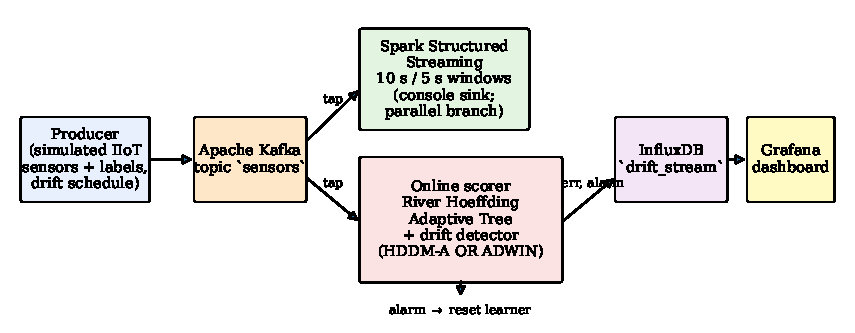
\includegraphics[width=0.92\textwidth]{figs/arch.pdf}
\caption{Pipeline architecture and data flow. The Spark branch is an optional parallel consumer and was not run.}
\label{fig:arch}
\end{figure*}

\section{Proposed Enhancement}
Error-rate detectors differ in what they are sensitive to: DDM and HDDM-A test a running mean of the error bit against its historical minimum, HDDM-W uses exponentially weighted averages, EDDM monitors the distance between consecutive errors, and ADWIN shrinks a window whenever two sub-windows have significantly different means~\cite{bifet2007}. We combine two detectors with different mechanisms:
\begin{equation}
\text{alarm}_t=\big(f_t\lor s_t\big)\land(t-t_{\text{last}}>R),
\end{equation}
where $f_t$ is HDDM-A, $s_t$ is ADWIN, $t_{\text{last}}$ is the previous emitted alarm and $R=500$ a refractory period. The OR rule raises recall because the two tests fire on different samples; the refractory period merges the burst of alarms that follows one drift.

\textbf{Change from the proposal.} The proposal planned to pair a fast detector (DDM or HDDM-W) with EDDM. That pairing, Paper 2's ADWIN/EDDM pair and an AND (confirmation) rule are all evaluated below as ablations; all of them performed worse than single detectors, which is why the final hybrid pairs HDDM-A with ADWIN. Two further variants isolate design choices: HDDM-A with the same refractory period but no fusion (HDDM-A+R500), and a hybrid whose ADWIN only reports \emph{increases} of the error rate (one-sided; ADWIN-up). ADWIN is two-sided, and in a deployment where a learner is reset, the falling error of the fresh learner is improvement, not drift.

\textbf{Selection bias.} The pairing and $R=500$ were chosen in exploratory runs on seeds 0--29, so results on those seeds are optimistic. A refractory sweep on separate seeds 1000--1019 (Table~\ref{tab:sweep}), a confirmatory run on untouched seeds 2000--2029 and the varied setting on seeds 3000--3099 check this. All detectors use River defaults.

\section{Implementation}
Python~3.14 with River~0.26.1, LightGBM~4.7.0, NumPy~2.5, SciPy~1.18, scikit-learn~1.9 and pandas~3.0. The infrastructure (\texttt{docker-compose.yml}) is Apache Kafka~3.7.0 in KRaft mode, InfluxDB~2.7 and Grafana~10.4.2, with \texttt{kafka-python} and \texttt{influxdb-client}.

\textbf{Synthetic drift streams.} Each stream is a binary error indicator whose error probability rises by an amplitude at each drift. Abrupt drift switches instantly; incremental drift ramps the probability linearly over the drift width; gradual drift draws each sample from the new concept with a linearly increasing probability. In the \emph{fixed} setting streams have 10\,000 samples, three drifts (2\,500/5\,000/7\,500), base error 0.10, amplitude 0.12 and width 500. In the \emph{varied} setting, which follows Paper 1 in varying stream size, number of drifts and drift duration and amplitude, each stream draws its length from \{5k, 10k, 20k\}, 1--4 drifts (at least twice the width apart), width from \{250, 500, 1000\}, base error from \{0.05, 0.10\} and amplitude from \{0.05, 0.10, 0.15\}. Each setting has the same number of streams per drift type.

\textbf{Simulated IIoT stream.} 20\,000 samples with eight features and a label from a linear boundary plus an interaction term and noise. The boundary changes abruptly at 5\,000 and 10\,000 and gradually over 1\,500 samples from 15\,000.

\textbf{IoTID20 and CICIDS2017.} We use the samples published with Paper 2 (6\,252 IoTID20 flows, 94\% attacks; 14\,155 CICIDS2017 flows, 19\% attacks) with binary labels, dropping flow and IP identifiers and the timestamp. In \emph{natural order} the streams drift (strongly in CICIDS2017), but drift positions are unknown. To score detection we also build \emph{injected-drift} streams: the rows are shuffled with a seed, which removes the natural drift, and at three onsets spread over the post-training part the five most important features (by a LightGBM fit on the training part) swap columns with random other features, a new remapping per drift. This mimics a sensor or firmware remapping: the data stay real while $P(y\mid x)$ as seen by the model changes. Drifts 1 and 2 are abrupt and drift 3 is gradual over 500 rows. The static model's error rises from under 1\% to 5--15\% at the onsets.

\textbf{Downstream learners.} The first 1\,000 samples train LightGBM. Evaluation is prequential in micro-batches of 25. For drift-triggered variants the detector receives each error bit; after an alarm the pipeline waits 300 samples and retrains on the post-alarm samples only (at most 500), so the new model does not learn the old concept; the detector is then reset. River's Adaptive Random Forest (5 trees) and Hoeffding Adaptive Tree are online baselines. Every stream with drift labels is run with 10 seeds.

\begin{table}[t]
\caption{Key configuration choices.}
\label{tab:cfg}
\centering\footnotesize\setlength{\tabcolsep}{3pt}
\begin{tabular}{@{}p{0.32\columnwidth}p{0.62\columnwidth}@{}}
\toprule
Item & Setting\\
\midrule
Synthetic, fixed & 10\,000 samples, 3 drifts, error 0.10 $+$0.12 per drift, width 1 or 500; seeds 0--29 and 2000--2029\\
Synthetic, varied & random length, drifts, width, base, amplitude; seeds 3000--3099 (300 streams)\\
Tolerance window & $[t,\,t+w+300)$, capped at next onset\\
Hybrid & HDDM-A OR ADWIN, refractory $R=500$\\
LightGBM & 80 trees, learning rate 0.1, 15 leaves, single thread\\
Retraining & wait 300 after alarm; train on post-alarm data ($\le$500); reset detector\\
Injected drift & shuffle rows; swap top-5 features at 25/50/75\% of stream\\
Live pipeline & Hoeffding Adaptive Tree; warm-up 300 records; replay 1\,000 records/s\\
\bottomrule
\end{tabular}
\end{table}

\section{Experimental Setup and Results}
\textbf{Scoring.} A drift onset $t$ is detected if the first alarm falls in $[t,\,t+w+300)$ and before the next onset, where $w$ is the drift width. Every other alarm is a false alarm and an unmatched onset is a miss. We report F1, mean delay over detected drifts, \emph{penalised} delay (a miss counts as the whole window), false alarms per 1\,000 samples, per-sample time and peak allocated memory. Detectors are compared with the Friedman test over streams, the Nemenyi critical difference (CD)~\cite{demsar2006}, and Holm-corrected Wilcoxon signed-rank tests of the hybrid against each other detector, which are more powerful than Nemenyi for comparisons with one method.

\textbf{Detector benchmark, fixed setting.} Table~\ref{tab:overall} and Fig.~\ref{fig:bench} give the results. The Friedman test rejects equal F1 ($\chi^2=586.6$, $p<10^{-100}$; CD 1.76 for $k=12$, which includes the one-sided variant; it gives identical results on these streams because they contain only error increases). The hybrid has the best F1 (0.733) and rank (3.23), ahead of HDDM-A (0.672) and ADWIN (0.611). The Wilcoxon tests find it significantly better than HDDM-A ($p=0.042$) and ADWIN ($p=0.0002$) but not than HDDM-A+R500 ($p=0.22$): of the 0.061 F1 gain over HDDM-A, 0.008 comes from the refractory period alone. The fusion's real effect is higher recall (0.759 vs 0.689) at a lower false-alarm rate. On the unseen seeds 2000--2029 the ordering repeats (hybrid 0.786, HDDM-A+R500 0.734, HDDM-A 0.723, ADWIN 0.641), with the same significance pattern ($p=0.021$ vs HDDM-A, $0.22$ vs HDDM-A+R500).

\begin{table}[t]
\caption{Detector results, fixed setting (90 streams, seeds 0--29). FA = false alarms per 1\,000 samples; delay in samples (over detected drifts / penalised); time in $\mu$s per sample; mem = peak kB; rank = Friedman mean rank on F1.}
\label{tab:overall}
\centering\footnotesize\setlength{\tabcolsep}{2.5pt}
\begin{tabular}{@{}lrrrrrrr@{}}
\toprule
Detector & F1 & FA & Delay & Pen. & $\mu$s & kB & Rank\\
\midrule
Hybrid OR(A,ADWIN) & 0.733 & 0.097 & 445 & 482 & 3.1 & 4.4 & 3.23\\
HDDM-A+R500 & 0.680 & 0.102 & 469 & 507 & 2.8 & 4.0 & 3.91\\
HDDM-A & 0.672 & 0.110 & 469 & 507 & 2.7 & 5.2 & 4.12\\
ADWIN & 0.611 & 0.117 & 488 & 534 & 0.2 & 0.7 & 4.56\\
HDDM-W & 0.464 & 0.357 & 317 & 425 & 2.1 & 4.4 & 6.64\\
DDM & 0.418 & 0.278 & 451 & 522 & 0.4 & 0.8 & 7.21\\
AND(HDDM-W,EDDM) & 0.417 & 0.390 & 346 & 458 & 2.5 & 4.7 & 7.31\\
AND(HDDM-W,ADWIN) & 0.370 & 0.080 & 536 & 595 & 2.4 & 4.5 & 8.17\\
OR(ADWIN,EDDM) & 0.347 & 0.941 & 276 & 303 & 0.6 & 1.4 & 8.30\\
OR(HDDM-W,EDDM) & 0.223 & 2.087 & 182 & 191 & 2.5 & 4.9 & 10.11\\
EDDM & 0.134 & 3.784 & 180 & 206 & 0.3 & 1.4 & 11.23\\
\bottomrule
\end{tabular}
\end{table}

\begin{figure*}[t]
\centering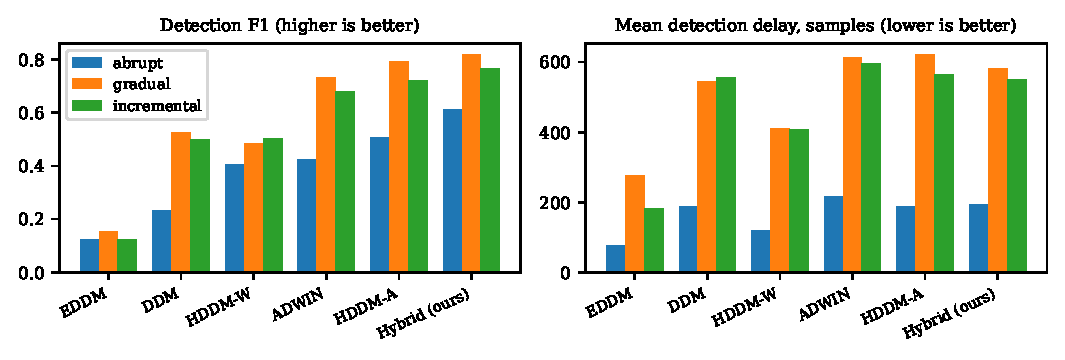
\includegraphics[width=0.95\textwidth]{figs/bench.pdf}
\caption{Detection F1 and mean detection delay by drift type, fixed setting.}
\label{fig:bench}
\end{figure*}

Per drift type (Table~\ref{tab:kind}), the hybrid's advantage over HDDM-A is largest for abrupt drift (F1 0.613 vs 0.505). EDDM reacts fastest (77--276 samples) but raises 3.4--4.1 false alarms per 1\,000 samples. On penalised delay the order is roughly the reverse of F1: EDDM-based detectors are fastest, then HDDM-W, then the hybrid, which is faster than HDDM-A, DDM and ADWIN ($p<0.001$ each).

\begin{table}[t]
\caption{F1 / mean delay (samples) by drift type, fixed setting.}
\label{tab:kind}
\centering\small
\begin{tabular}{@{}lccc@{}}
\toprule
Detector & Abrupt & Gradual & Incremental\\
\midrule
EDDM & 0.124 / 77 & 0.153 / 276 & 0.125 / 182\\
DDM & 0.231 / 188 & 0.524 / 545 & 0.498 / 556\\
HDDM-W & 0.404 / 119 & 0.485 / 411 & 0.503 / 408\\
ADWIN & 0.422 / 217 & 0.733 / 615 & 0.678 / 596\\
HDDM-A & 0.505 / 188 & 0.792 / 622 & 0.719 / 566\\
Hybrid & 0.613 / 193 & 0.819 / 583 & 0.767 / 551\\
\bottomrule
\end{tabular}
\end{table}

\textbf{Varied setting.} Over 300 streams with varied settings (Table~\ref{tab:varied}) all F1 values fall, mainly because small drifts (amplitude 0.05) are hard for every detector (F1 $\le$0.30). The hybrid is still first (0.591, rank 4.30) but ADWIN is now second (0.550, rank 4.79) and HDDM-A drops to 0.483. The hybrid is significantly better than HDDM-A and every other detector ($p<10^{-4}$) except ADWIN ($p=0.28$; rank gap 0.49 below the CD of 0.96). Its penalised delay (524) is lower than ADWIN's (557) and HDDM-A's (582).

\begin{table}[t]
\caption{Varied setting (300 streams): F1 overall and by drift amplitude, penalised delay, Friedman rank on F1 (CD 0.96).}
\label{tab:varied}
\centering\footnotesize\setlength{\tabcolsep}{3pt}
\begin{tabular}{@{}lrrrrrr@{}}
\toprule
Detector & F1 & 0.05 & 0.10 & 0.15 & Pen. & Rank\\
\midrule
Hybrid OR(A,ADWIN) & 0.591 & 0.234 & 0.617 & 0.934 & 524 & 4.30\\
ADWIN & 0.550 & 0.171 & 0.601 & 0.880 & 557 & 4.79\\
HDDM-A & 0.483 & 0.188 & 0.433 & 0.862 & 582 & 5.53\\
DDM & 0.323 & 0.159 & 0.362 & 0.442 & 582 & 7.13\\
OR(ADWIN,EDDM) & 0.279 & 0.292 & 0.254 & 0.300 & 342 & 6.29\\
HDDM-W & 0.255 & 0.115 & 0.269 & 0.383 & 584 & 7.42\\
EDDM & 0.132 & 0.166 & 0.117 & 0.119 & 276 & 8.59\\
\bottomrule
\end{tabular}
\end{table}

\textbf{Refractory sweep.} Table~\ref{tab:sweep} shows the sweep on seeds 1000--1019: F1 rises steadily with $R$ while delay stays near 424 samples, so $R=500$ is not the optimum of the range and was not selected from this sweep.

\begin{table}[t]
\caption{Refractory-period sweep of the hybrid on seeds 1000--1019 (60 streams, fixed setting).}
\label{tab:sweep}
\centering\small
\begin{tabular}{@{}rccc@{}}
\toprule
$R$ & F1 & Delay & FA / 1\,000\\
\midrule
100 & 0.634 & 424 & 0.215\\
200 & 0.702 & 424 & 0.145\\
300 & 0.722 & 424 & 0.125\\
500 & 0.755 & 424 & 0.093\\
800 & 0.775 & 424 & 0.075\\
\bottomrule
\end{tabular}
\end{table}

\textbf{Negative results.} Every fusion involving EDDM inherited its false-alarm rate: OR(HDDM-W,EDDM), the proposal's pairing, reached F1 0.223 and Paper 2's OR(ADWIN,EDDM) 0.347, both below ADWIN alone. Confirmation (AND) fusion lowered recall (0.31 for HDDM-W/ADWIN) and lengthened delay while barely reducing false alarms.

\textbf{Downstream adaptation.} Table~\ref{tab:down} and Fig.~\ref{fig:down} summarize the prequential study. On the simulated stream a static LightGBM falls to 0.60 accuracy, and every drift-triggered variant recovers to 0.82--0.84 (hybrid $0.834\pm0.021$); the online Hoeffding Adaptive Tree is the most accurate (0.848). The hybrid detects the true drifts well (detection F1 0.96, delay 207), close to ADWIN (0.99, 221) and HDDM-A (0.94, 246), while EDDM causes 47 alarms and 26 retrains for three drifts and DDM 9 alarms. On the injected-drift IoTID20 and CICIDS2017 streams retraining again helps (CICIDS2017 attack F1 0.64 static vs 0.91--0.93 retrained), but detection F1 is low for all detectors (0.05--0.39), because the error rises only to a few percent. On these streams HDDM-A rarely fires, so the hybrid behaves exactly like ADWIN. In natural order IoTID20 is essentially stationary: the static model reaches 0.995, the HDDM-A, ADWIN, EDDM and hybrid triggers correctly stay silent, and DDM's 15 false alarms cost accuracy. CICIDS2017 in natural order drifts strongly: the static model's attack F1 collapses to 0.016, retraining gives 0.73--0.89 (DDM best, with 40 alarms), and River ARF reaches 0.962.

\begin{table}[t]
\caption{Downstream results, mean of 10 seeds (natural order: one run). Sim = simulated IIoT accuracy; IoT, CIC = IoTID20, CICIDS2017 with injected drift (accuracy / attack F1); CIC-nat = CICIDS2017 natural order (attack F1).}
\label{tab:down}
\centering\footnotesize\setlength{\tabcolsep}{2.5pt}
\begin{tabular}{@{}lrrrr@{}}
\toprule
Strategy & Sim & IoT & CIC & CIC-nat\\
\midrule
Static LightGBM & 0.603 & 0.947 / 0.972 & 0.895 / 0.644 & 0.016\\
+ DDM & 0.836 & 0.974 / 0.986 & 0.967 / 0.910 & 0.895\\
+ HDDM-A & 0.831 & 0.955 / 0.977 & 0.966 / 0.905 & 0.733\\
+ ADWIN & 0.825 & 0.971 / 0.985 & 0.969 / 0.916 & 0.738\\
+ EDDM & 0.840 & 0.974 / 0.986 & 0.974 / 0.931 & 0.786\\
+ Hybrid (ours) & 0.834 & 0.971 / 0.985 & 0.969 / 0.916 & 0.756\\
River ARF & 0.816 & 0.971 / 0.985 & 0.962 / 0.892 & 0.962\\
River HAT & 0.848 & 0.947 / 0.973 & 0.877 / 0.576 & 0.879\\
\bottomrule
\end{tabular}
\end{table}

\begin{figure*}[t]
\centering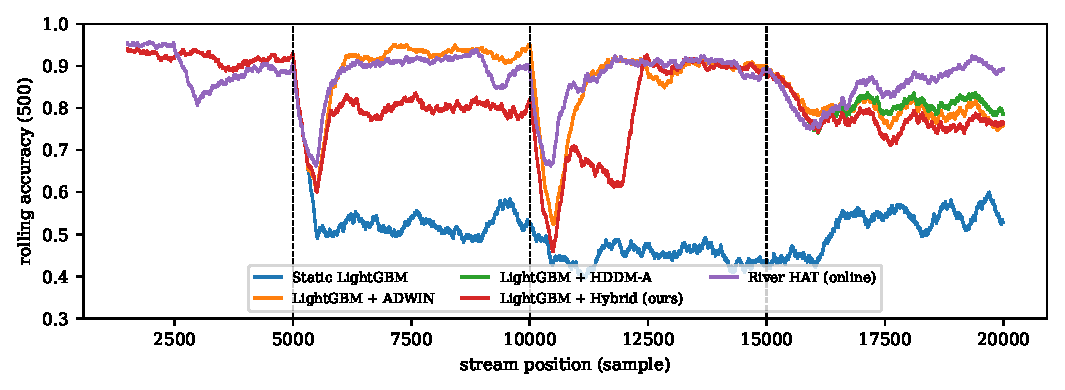
\includegraphics[width=0.95\textwidth]{figs/downstream.pdf}
\caption{Rolling prequential accuracy (window 300, seed 0). Dashed lines mark drift onsets. On IoTID20 the ADWIN and hybrid curves coincide.}
\label{fig:down}
\end{figure*}

\textbf{Live pipeline.} We streamed the 20\,000-record simulated stream through Kafka into the online scorer and InfluxDB (Fig.~\ref{fig:live}), with all points visible in Grafana. At an offered 1\,000 records/s the consumer processed 805 records/s with a median end-to-end latency of 3.1\,ms (95th percentile 20\,ms) for the hybrid and 2.2\,ms (7.4\,ms) for the one-sided variant. With the producer uncapped, the consumer's capacity was 824 records/s, and beyond it records queue in Kafka (median latency 12\,s). The limit is the single-threaded Python consumer with one synchronous InfluxDB write per record, not Kafka. The alarms were identical to an in-process run. The two-sided hybrid raised alarms at 2\,503, 5\,017, 10\,011, 14\,247 and 18\,803 (F1 0.50, three false alarms), the one-sided hybrid at 2\,503, 5\,017, 10\,011 and 15\,335 (F1 0.86, one false alarm, the same as HDDM-A alone). The alarm at 2\,503, raised by every detector, follows a real rise in the tree's error with no change in the data.

\begin{figure}[t]
\centering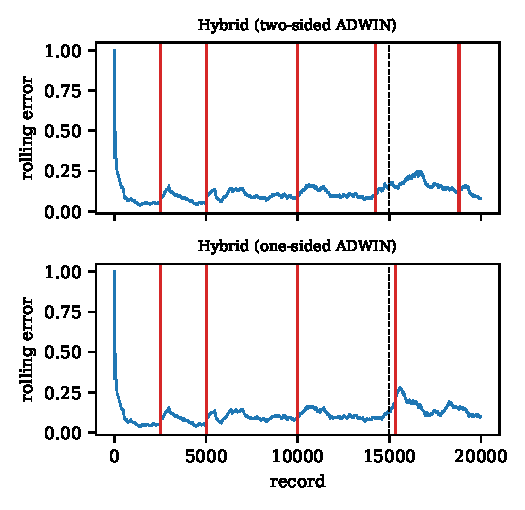
\includegraphics[width=\columnwidth]{figs/live.pdf}
\caption{Live Kafka run: rolling error (blue), alarms (red) and true drift onsets (dashed; the first two coincide with alarms).}
\label{fig:live}
\end{figure}

\section{Discussion and Inferences}
\textbf{Answer to the research question.} No single detector wins on every axis. Mean-based detectors (HDDM-A, ADWIN) give the best accuracy--false-alarm balance; EDDM and HDDM-W react fastest but at many times the false-alarm rate. Fusing HDDM-A and ADWIN with an OR rule and a refractory period gives the best F1 in every synthetic setting and a lower penalised delay than either component, for about 3\,$\mu$s and 4\,kB per stream, negligible next to a Kafka hop. The gain is robust against HDDM-A but not against ADWIN when stream settings vary, so the claim we can support is ``at least as good as the best single detector, and more robust across settings than either component''.

\textbf{Relation to base paper 1.} Sakurai et al.\ report EDDM as the most accurate detector and HDDM-W as the best trade-off. We reproduce the qualitative finding that no detector dominates, and HDDM-W does have lower delay than DDM and HDDM-A, but EDDM has the lowest F1 in both of our settings. We attribute this to our scoring rule (every extra alarm is a false alarm), the use of untuned defaults, and our own generator; we do not claim to reproduce their ranking.

\textbf{Downstream.} Drift-triggered retraining is clearly worth doing when drift is real (simulated stream, CICIDS2017), and well-behaved detectors cost nothing when it is not (IoTID20). However, better detection F1 did not translate into better accuracy. On streams with frequent class-prior shifts, as in CICIDS2017, a ``noisy'' trigger such as DDM retrains more often and benefits, while online learners with built-in adaptation (River ARF, HAT) are competitive or better. Detection quality and adaptation quality should therefore be evaluated separately.

\textbf{Deployment considerations.} A detector fed by a learner that has just been reset sees a falling error rate, and two-sided tests such as ADWIN treat improvement as change. The warm-up guard and one-sided ADWIN together removed this class of alarm in the live run. In a plant, an alarm should trigger review or a controlled retrain rather than an unattended model swap, so alarm precision matters more than delay.

\textbf{Threats to validity.} (1) Detector benchmarks use synthetic Bernoulli error streams; real classifier errors are autocorrelated. (2) The hybrid was designed on seeds 0--29 and only it was tuned, while baselines use River defaults; the unseen-seed and varied runs reduce but do not remove this advantage. (3) The 300-sample margin and the drift amplitudes are our choices. (4) Drift in IoTID20 and CICIDS2017 is injected by feature remapping, which is one kind of real drift; natural-order runs have no ground truth. (5) We use the published dataset samples, not the full datasets. (6) The live run uses one machine, one consumer and the simulated stream; the Spark branch was not run.

\section{Reproducibility}
\texttt{python -m drift.benchmark} (fixed, seeds 0--29), \texttt{-{}-start 2000 -{}-out results\_heldout} (unseen seeds), \texttt{-{}-varied -{}-seeds 100 -{}-start 3000 -{}-out results\_varied}, \texttt{python -m drift.tune\_hybrid}, \texttt{python -m drift.adaptive} (downstream, all datasets), \texttt{python -m streaming.run\_local}, and \texttt{docker compose up -d}, \texttt{python -m streaming.consumer -{}-max 20000}, \texttt{python -m streaming.producer -{}-rate 1000} for the live path. Unit tests: \texttt{pytest tests}. All seeds are fixed; timings depend on the machine.

\section{Conclusion and Future Work}
We benchmarked five drift detectors and six fusion variants on 480 synthetic streams, studied drift-triggered retraining on simulated and real IIoT data, and ran a live Kafka monitoring pipeline. An OR-fusion of HDDM-A and ADWIN with a refractory period gave the best detection F1 in every setting, significantly better than HDDM-A and tied with ADWIN when settings vary, while EDDM-based and confirmation fusions failed. Retraining recovered most of the accuracy lost to drift, but detector quality alone did not decide downstream accuracy. Future work: tune all detectors on equal footing, evaluate the full datasets and other kinds of injected drift, batch InfluxDB writes and partition the topic to scale the consumer, and route Spark window features into the detector.

\begin{thebibliography}{99}
\bibitem{gama2014survey} J. Gama, I. \v{Z}liobait\.{e}, A. Bifet, M. Pechenizkiy, and A. Bouchachia, ``A survey on concept drift adaptation,'' \emph{ACM Comput. Surv.}, vol. 46, no. 4, pp. 1--37, 2014.
\bibitem{sakurai2023} G. Y. Sakurai, J. F. Lopes, B. B. Zarpel\~ao, and S. Barbon Junior, ``Benchmarking change detector algorithms from different concept drift perspectives,'' \emph{Future Internet}, vol. 15, no. 5, p. 169, 2023.
\bibitem{yang2023msana} L. Yang and A. Shami, ``A multi-stage automated online network data stream analytics framework for IIoT systems,'' \emph{IEEE Trans. Ind. Informat.}, vol. 19, no. 2, pp. 2107--2116, 2023.
\bibitem{yang2021lightweight} L. Yang and A. Shami, ``A lightweight concept drift detection and adaptation framework for IoT data streams,'' \emph{IEEE Internet Things Mag.}, vol. 4, no. 2, pp. 96--101, 2021.
\bibitem{gama2004} J. Gama, P. Medas, G. Castillo, and P. Rodrigues, ``Learning with drift detection,'' in \emph{Proc. SBIA}, LNCS 3171, 2004, pp. 286--295.
\bibitem{baena2006} M. Baena-Garc\'ia \emph{et al.}, ``Early drift detection method,'' in \emph{Proc. 4th Int. Workshop Knowledge Discovery from Data Streams}, 2006.
\bibitem{frias2015} I. Fr\'ias-Blanco \emph{et al.}, ``Online and non-parametric drift detection methods based on Hoeffding's bounds,'' \emph{IEEE Trans. Knowl. Data Eng.}, vol. 27, no. 3, pp. 810--823, 2015.
\bibitem{bifet2007} A. Bifet and R. Gavald\`a, ``Learning from time-changing data with adaptive windowing,'' in \emph{Proc. SIAM Int. Conf. Data Mining}, 2007, pp. 443--448.
\bibitem{montiel2021} J. Montiel \emph{et al.}, ``River: machine learning for streaming data in Python,'' \emph{J. Mach. Learn. Res.}, vol. 22, no. 110, pp. 1--8, 2021.
\bibitem{ke2017} G. Ke \emph{et al.}, ``LightGBM: A highly efficient gradient boosting decision tree,'' in \emph{Proc. NeurIPS}, 2017, pp. 3146--3154.
\bibitem{demsar2006} J. Dem\v{s}ar, ``Statistical comparisons of classifiers over multiple data sets,'' \emph{J. Mach. Learn. Res.}, vol. 7, pp. 1--30, 2006.
\end{thebibliography}
\end{document}
